
%%%%%%%%%%%%%%%%%%%%%%% file typeinst.tex %%%%%%%%%%%%%%%%%%%%%%%%%
%
% This is the LaTeX source for the instructions to authors using
% the LaTeX document class 'llncs.cls' for contributions to
% the Lecture Notes in Computer Sciences series.
% http://www.springer.com/lncs       Springer Heidelberg 2006/05/04
%
% It may be used as a template for your own input - copy it
% to a new file with a new name and use it as the basis
% for your article.
%
% NB: the document class 'llncs' has its own and detailed documentation, see
% ftp://ftp.springer.de/data/pubftp/pub/tex/latex/llncs/latex2e/llncsdoc.pdf
%
%%%%%%%%%%%%%%%%%%%%%%%%%%%%%%%%%%%%%%%%%%%%%%%%%%%%%%%%%%%%%%%%%%%


\documentclass[runningheads,a4paper]{llncs}

\usepackage{amssymb}
\setcounter{tocdepth}{3}
\usepackage{graphicx}
\usepackage{booktabs}
\usepackage{float}
\usepackage{url}
\urldef{\mailsa}\path|{rafael.possas, ying.zhou}@sydney.edu.au|    
\newcommand{\keywords}[1]{\par\addvspace\baselineskip
\noindent\keywordname\enspace\ignorespaces#1}

\begin{document}

\mainmatter  % start of an individual contribution

% first the title is needed
\title{Effectiveness of Adversarial Attacks on Class-Imbalanced Convolutional Neural Networks}
\titlerunning{Effectiveness of Adversarial Attacks on Class-Imbalanced CNNs}
% a short form should be given in case it is too long for the running head

% the name(s) of the author(s) follow(s) next
%
% NB: Chinese authors should write their first names(s) in front of
% their surnames. This ensures that the names appear correctly in
% the running heads and the author index.
%
\author{Rafael Possas, Ying Zhou}
%
\authorrunning{Rafael Possas, Ying Zhou}
% (feature abused for this document to repeat the title also on left hand pages)

% the affiliations are given next; don't give your e-mail address
% unless you accept that it will be published
\institute{School of Information Technologies, University Of Sydney, Camperdown, NSW \\
\mailsa\\
\url{https://sydney.edu.au}}

%
% NB: a more complex sample for affiliations and the mapping to the
% corresponding authors can be found in the file "llncs.dem"
% (search for the string "\mainmatter" where a contribution starts).
% "llncs.dem" accompanies the document class "llncs.cls".
%

\maketitle


\begin{abstract}
Convolutional neural networks (CNNs) performance has increased considerably in the last couple of years. However, as with most machine learning methods, these networks suffer from the data imbalance problem - when the underlying training dataset is comprised of an unequal number of samples for each label/class. Such imbalance enforces a phenomena known as domain shift that causes the model to have poor generalisation when presented with previously unseen data. Recent research has focused on a technique called \textit{gradient sign} that intensifies domain shift in CNNs by modifying inputs to deliberately yield erroneous model outputs, while appearing unmodified to human observers. Several commercial systems rely on image recognition techniques to perform well. Therefore, adversarial attacks poses serious threats to their integrity. In this work we present an experimental study that sheds light on the link between adversarial attacks, imbalanced learning and transfer learning. Through a series of experiments we evaluate the \textit{fast gradient sign method} on class imbalanced CNNs, linking model vulnerabilities to the characteristics of its underlying training set and internal model knowledge.
\keywords{convolutional neural networks, adversarial examples, gradient sign, imbalanced training, transfer learning}
\end{abstract}


\section{Introduction}


Convolutional neural networks (CNNs) are a class of non-linear machine learning algorithms known for its state of the art performance on datasets with spatial structure. To date, not much research has been done on adversarial attacks against CNNs - a process on which inputs are changed to manipulate the algorithm outputs. The motivation for adversarial robustness comes largely from being able to shield image recognition systems from behaving unexpectedly. Experimental demonstrations of the effectiveness of adversarial attacks were carried out mainly by \cite{billovits,goodfellow2014,papernot2016} and have heightened the need for improvement on the current state of CNNs techniques. Developing robustness to such attacks has become of the utmost importance as many commercial applications are based on the same small group of models.

Domain shift or dataset shift \cite{Quionero} is also a well known cause for low performance of several machine learning algorithms \cite{japkowicz2002class,krawczyk2016learning}. This happens when the joint distribution of inputs and outputs differs between training and testing stages, causing models to perform badly on unseen data. The adverse effect of domain shift is even worse on real world, as data distributions are often skewed and rarely contains enough information to learn all the required features of the data domain. Adversaries have been proven to more readily exploit domain shift \cite{Laskov2010,lowd2005}, and the question as to whether imbalanced training sets affects adversarial inputs performance on CNNs is still unanswered. 

The effectiveness of an adversarial attack also depends on the internal gradient information of the targeted model. As shown on Papernot et al (2016), attacks could be classified as both black-box and white-box. The former uses gradient information from a separate model, while the latter uses the target model gradient to generate adversarial inputs. While black-box attack is an approximation of the internal knowledge of the target model, the white-box uses the true representation of the feature space.

Currently, there is no empirical evidence on the effectiveness of adversarial attacks on class-imbalanced CNNs. We designed a set of experiments to investigate how both imbalanced training sets and the model's internal knowledge affects the robustness to such attacks. The main contributions of this work are as follows: 
\begin{enumerate}
	\item To shed new light on how CNNs trained on imbalanced datasets are affected by adversarial attacks
	\item Evaluate the impact of transfer learning on imbalanced CNNs and how classes with similar set of features react to the perturbation caused by the gradient sign method
\end{enumerate}

Section 2 of this paper discusses the related work in both CNNs, gradient sign methods, adversarial attacks and imbalanced/transfer learning. Section 3 provides details of the training models, imbalanced datasets and gradient sign methods used in our experiments. Section 4 presents the results on the under-sampled, over-sampled and balanced cases using both black/white-box attacks. Sections 5 is dedicated to drawing conclusions and providing directions to related future work.
\section{Related Work}


Previous work has shown that the high-dimensional non-linearities of convolutional neural networks \cite{lawrence1997face} creates adversarial pockets of space - places where data points can be placed in order to provide a wrong model output. By exploiting such characteristics, recent methods were able to deliberately create an adversary that produces an incorrect, high confidence prediction for an image without visible distortion \cite{papernot_thesis_2016}. This is achieved by adding intentional noise to each pixel of an image so as to fool the algorithm into predicting an incorrect label \cite{goodfellow2014,papernot2016transf,szegedy2013}.

The gradient sign method was introduced by Goodfellow et al. (2014) and has been used as the foundation of many of the experiments in adversarial attacks on CNNs. The results have shown that convolutional neural networks have linear behavior in very high dimensional spaces \cite{goodfellow2014}.  Most inputs were miss-classified not only by Goodfellow et. al (2014) experiments but by others as well \cite{billovits,papernot2016}.

The work of Papernot et al. (2016) has shown that one can use transfer learning to perform black-box attacks against CNNs \cite{papernot2016transf,yosinski2014transferable} and, thus, to intentionally force the model to predict specific labels. The combination of adversaries and transfer learning creates a threat vector for many state of the art methods. Attacks, however, depend on some specific internal information of the target model \cite{lowd2005,papernot2016transf}. For instance, the same model trained by two different configurations of the same dataset would have different gradients and thus, would provide different degrees of adversarial perturbations.

Techniques to overcome imbalanced learning have been developed for more general machine learning models. The work of Heibo et al \cite{he2008adasyn}, for instance, provides a technique for doing weighted sampling of minority classes to minimize the effect of imbalanced learning. Another approach could be to incorporate unsupervised clustering on synthetic data generation mechanism in order to avoid wrong generation of synthetic samples \cite{Barua2011}. More recent work has used a Bayesian framework to increase $l_2$ robustness to adversarial examples \cite{billovits}.

\section{Experiment Design}

Our experiments aims to investigate the relationships of the underlying learning structure of CNNs and the perturbation caused by gradient sign methods. In particular we focus on the investigation of how the gradient step from the sign method moves the points away from their distributions, and how this could be affected by both balanced and imbalanced training sets. This requires  class labels of the data set to be non-hierarchical so we can make better assumptions of their distributions. 

We use the CIFAR-10 data set \cite{krizhevsky_2009} in our experiment. CIFAR-10 data is visually rich and empowers the analysis between different class labels. The data set contains 32x32 images in 10 classes, each has 5,000 samples for training and 1,000 for testing. There is not much overlap nor hierarchical relationship between classes. Most CNNs experiments nowadays use the 2014 ImageNet dataset \cite{deng2009imagenet}. However, its hierarchically organized categories adds unnecessary complexity to the experiment design and hinders the analysis of the results (e.g. causality relationships).
\subsection{Network architecture and synthetic dataset imbalance}
\begin{figure}
	\centering
	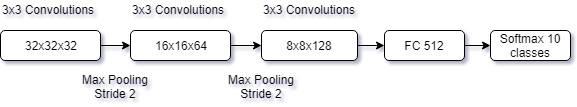
\includegraphics[height=2.0cm]{net_diagram.png}
	\caption{Adapted VGG Architecture}
	\label{fig:vgg_arch}
\end{figure}

\subsubsection{Network Architecture} All the experiments were performed using a modified VGGNet \cite{simonyan2014very} architecture as shown on figure \ref{fig:vgg_arch}. The two fully connected 4096 layers at the end were replaced by one single layer with 512 neurons and RELU activations. In addition, the total number of convolutions blocks and pooling layers were reduced to 3, with the first layer having 2 stacked convolution layers followed by a max pooling of stride 2x2 and the last two layers with 3 stacked convolutions also followed by a max pooling of stride 2x2. We have used RMSProp  \cite{bengiormsprop} as the optimisation technique with a learning rate of $10^{-4}$ and a decay $10^{-5}$. Figure~\ref{fig:conf_matrix_full} shows that our model has an overall accuracy of approximately 83\%, which is comparable to many state of the art models nowadays.

\begin{figure}
	\centering
	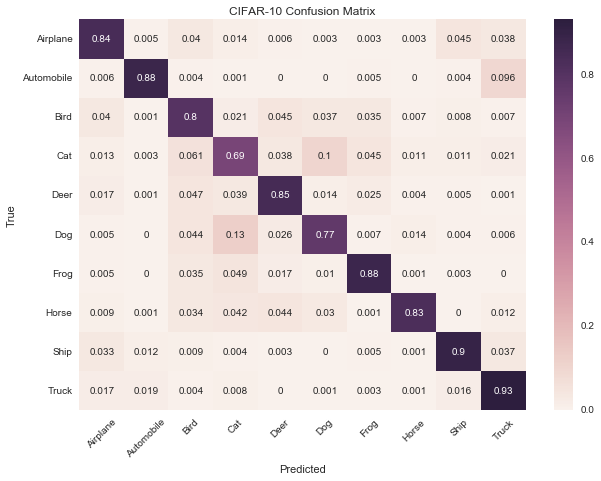
\includegraphics[height=6.0cm]{conf_matrix.png}
	\caption{Results of our adapted VGG architecture on the CIFAR-10 dataset shows comparable overall performance}
	\label{fig:conf_matrix_full}
\end{figure}

\subsubsection{Dataset imbalancing} As the CIFAR-10 dataset is not naturally imbalanced, we have artificially created two variations on which we trained the imbalanced models.  One dataset consists of a direct under-sample of the target class to 1,000 samples, and the other was changed using  an over-sampling of the target class (or an under-sampling of all other classes). We kept the number of samples for the target class at 5,000 while all other classes were reduced to 1,000 samples. For each class of the two different datasets configurations, a network was then trained until convergence using the same hyper-parameters as the balanced case. Each model was evaluated against a test set of 1,000 samples of the target class which was  perturbed by its own under/over-sampled model and the balanced model. The two sources of gradient information are referred as white-box and black-box attacks since the former has complete information of the model weights and biases while the latter uses an approximation of the same parameters. 

Both imbalanced models were separately tested for each class on white-box and black-box adversarial attacks. The white-box test was designed to investigate the vulnerability of class imbalance on adversarial examples while the black-box test is designed to verify the robustness on transfer learning environments. In total we evaluated 50 different combinations: 20 for each different imbalanced dataset (same model gradient and balanced model gradient) and 10 for the balanced model using its own gradients on each class. Figure~\ref{fig:acc_graph} shows the accuracy for the models without any perturbation. It can be seen that the individual class accuracy for the under-sampled case is generally reduced while the same metric is increased on the over-sampling model. 


\subsection{Gradient sign methods}

The gradient sign is a method that uses internal gradient information to create directed perturbation to input data. The resulting label will be different whether one adds or subtracts noise according to equations 1 and 2. 

\begin{equation}
C(x + \delta)\approx C(x) + \epsilon * sign(\nabla C)
\end{equation}
\begin{equation}
C(x + \delta)\approx C(x) - \epsilon * sign(\nabla C)
\end{equation}

The gradient sign equation has a simple interpretation. The main goal is to add a change $\delta$ into each pixel of the image so as to make that image closer to the chosen label on which we extracted the gradient from the source model. The sign on our $\nabla C$ indicates that we are only interested on the direction of the gradient while the $\epsilon$ controls the magnitude of the step.

\begin{figure}
	\centering
	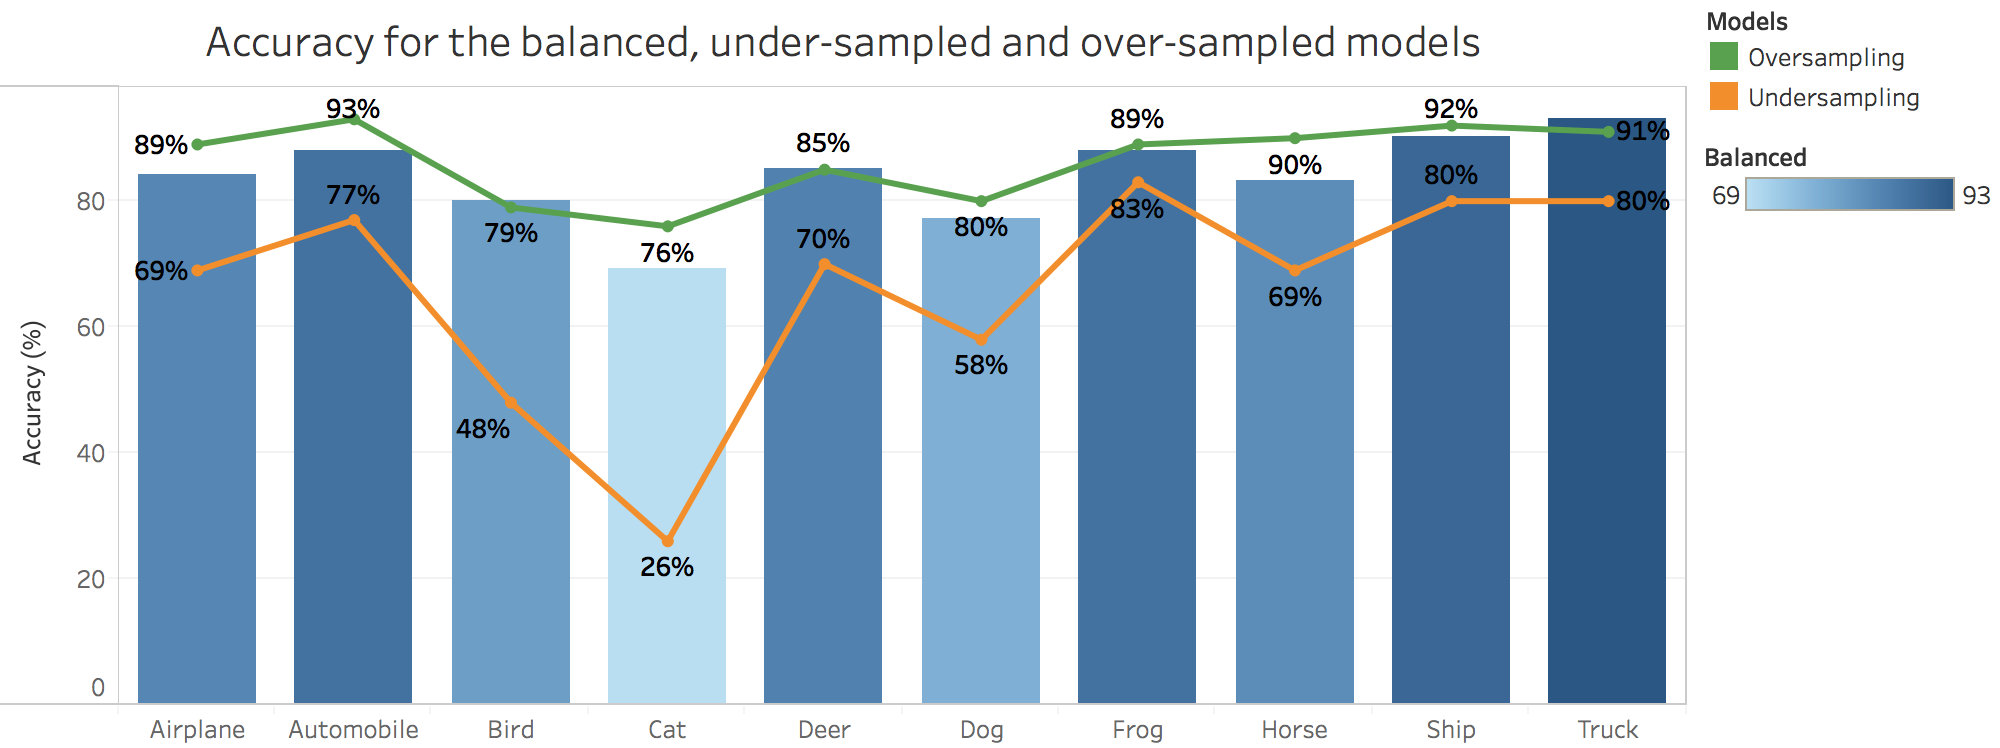
\includegraphics[height=3.5cm]{graph_non_pert.png}
	\caption{Individual class accuracy for under-sampled, over-sampled case on the CIFAR-10 modified dataset shows a decrease in accuracy for classes with lower number of samples}
	\label{fig:acc_graph}
\end{figure}

Suppose the current true label of the class is selected as a gradient candidate, adding noise would mean that we increase the cost function of our input while subtracting noise is the same as minimizing our loss function even further. 
The equations above are usually referred as ascent and descent methods

Perturbations could also be applied by two variations of the gradient sign method. While the fast gradient sign method applies a single perturbation to the input, the iterative gradient sign method performs the same perturbation a chosen number of times iteratively \cite{goodfellow2014}. Figure~\ref{fig:fgsm_craft} shows an example of adversarial created using the fast method.



\begin{figure}
	\centering
	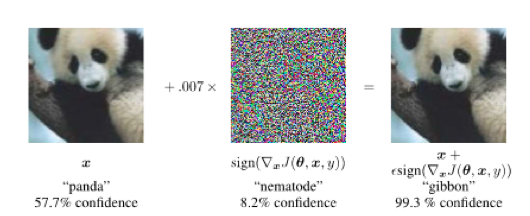
\includegraphics[height=2.5cm]{panda.png}
	\caption{Adversarial example crafting with fast gradient sign \cite{goodfellow2014}.}
	\label{fig:fgsm_craft}
\end{figure}

In order to enforce consistency throughout our experiments, we have chosen the true sample label as the backpropagated gradient along with the fast gradient sign ascent method. The intuition behind this choice is that we look to increase the cost function of the target class by moving away from the current true label. The $\epsilon$ value chosen was 0.01 as it provided the best trade-off between misclassification rate and the amount of visible change applied to the input image.


\section{Results}
We use the results of the balanced model on adversarial attacks as the baseline to evaluate whether imbalanced CNNs are more or less vulnerable to adversarial learning. Table~\ref{tbl:results} shows that the accuracy for all classes is drastically reduced when the balanced model is presented with adversarial examples. Models with under-sampled datasets were even more vulnerable than balanced models. Figure~\ref{fig:relative_difference} shows the relative difference for all the three different models (balanced, under-sampled and over-sampled). Values were calculated by finding the difference between the perturbed accuracy and the non-perturbed accuracy of each class model. They represent the percentage on which the initial accuracy was reduced. The under-sampled model had the higher relative difference on average, which shows that the imbalanced nature of the dataset ended-up increasing the vulnerability of the model.

\begin{figure}
	\centering
	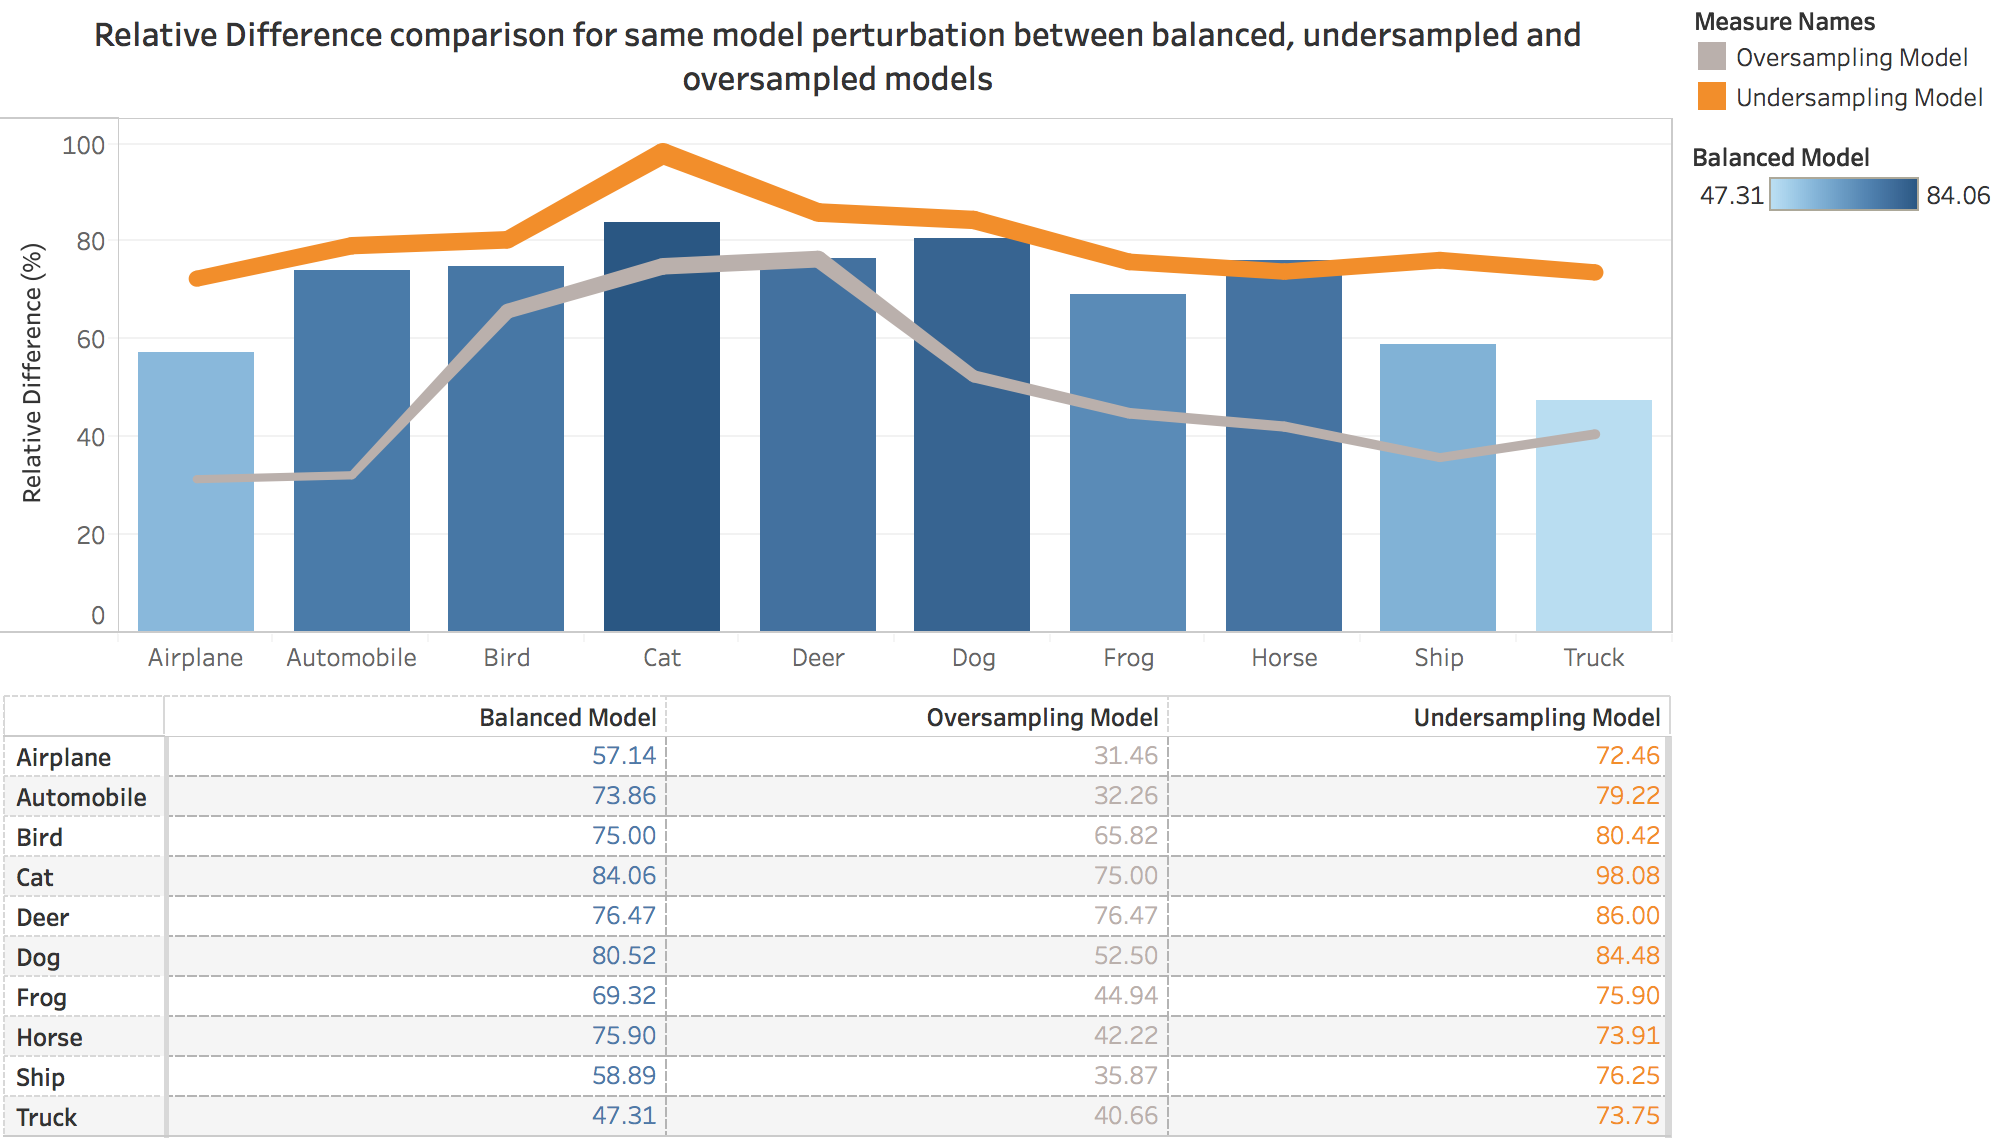
\includegraphics[height=3.5cm]{rel_diff_graph.png}
	\caption{Relative difference for each model. Higher numbers means more vulnerability}
	\label{fig:relative_difference}
\end{figure}


Perturbation on the over-sampling case had a weaker effect, as the small push caused by our $\epsilon$ was not enough to move points to outside of their distributions. Objects of the over-sampled classes would need bigger steps in order to successfully create an adversary that leads to a wrong classification label. Accuracy for most of the over-sampling cases was around 45\% and the relative difference was the lowest of all three models, which shows robustness of the target over-sampled class. 


Class imbalanced models are naturally affected by the false positive and false negative trade off shown on figure~\ref{fig:class_dist}. The decision boundaries on such models favor the class with more samples and, hence, increases the accuracy for this class while decreasing for the other classes. The area under the curve for misclassified examples on the under-sampled distribution is bigger, and it is caused by the suboptimal exploration of feature space of that class. This effect is exploited by adversaries as there is an increase on the misclassification rate of distributions with lower amplitude.
\begin{table}
	\centering	
	\begin{tabular}{lccccc}
		\toprule
		&\multicolumn{2}{c}{Black-box}
		&\multicolumn{3}{c}{White-box}
		\\\cmidrule(r){2-3}\cmidrule(l){4-6}
		Class Label &Undersample &Oversample &Balanced &Undersample &Oversample \\
		\midrule
		0 - Airplane &60\%& 87\% &36\%& 19\%    & 61\% \\
		1 - Automobile &64\%& 91\% &23\%& 16\%    & 63\% \\
		2 - Bird &38\%& 73\% &20\%& 9.4\%    & 27\% \\
		3 - Cat &21\%& 72\% &11\%& 0.5\%    & 19\% \\
		4 - Deer &58\%& 80\% &20\%& 9.8\%    & 20\% \\
		5 - Dog &47\%& 76\% &15\%& 9\%    & 38\% \\
		6 - Frog &76\%& 88\% &27\%& 20\%    & 49\% \\
		7 - Horse &59\%& 88\% &20\%& 18\%    & 52\% \\
		8 - Ship &69\%& 89\% &37\%& 19\%    & 59\% \\
		9 - Truck &46\%& 87\% &49\%& 21\%    & 54\% \\
		\bottomrule
		\hfill
	\end{tabular}
	\caption{Results for the two different sources of perturbations along with the two different imbalanced datasets. Under-sampling intensifies adversarial attack while over-sampling increases model robustness}
	\label{tbl:results}
\end{table}
The increased number of samples of the over-sampled label causes the model to perform a trade-off when optimizing its loss function. For instance, the decision boundary would be chosen in order to minimize the total error of the model. The cost function is lower when the decision boundary minimizes the misclassification of the majority class as there is a higher number of samples. The choice of a biased decision boundary could be one of the factors explaining the higher resilience of over-sampled models.

\subsection{Transfer learning and overlapping distributions}

\subsubsection{Transfer learning} The use of a different model gradient (black-box) for creating adversaries has shown less effective when compared to the same model (white-box) attack. As the overall gradient have not only different direction but also magnitudes, the system has proven to be more robust to the attack. The experiment reveals that although the gradient sign method is quite effective for fooling CNN models it does require a good amount of knowledge from the underlying training parameters so as to unleash its full potential. Attacking an under-sampled/over-sampled model with the gradient of the balanced model did not show to be as effective as using the same model's gradient. The average accuracy of an under-sampled model attack with adversaries generated from a different model was 53.8\% while the same metric was 25.8\% for the same model attack. Even that our training samples are within the same data domain, there are still huge differences on the gradients learned from the model. 
\begin{figure}
	\centering
	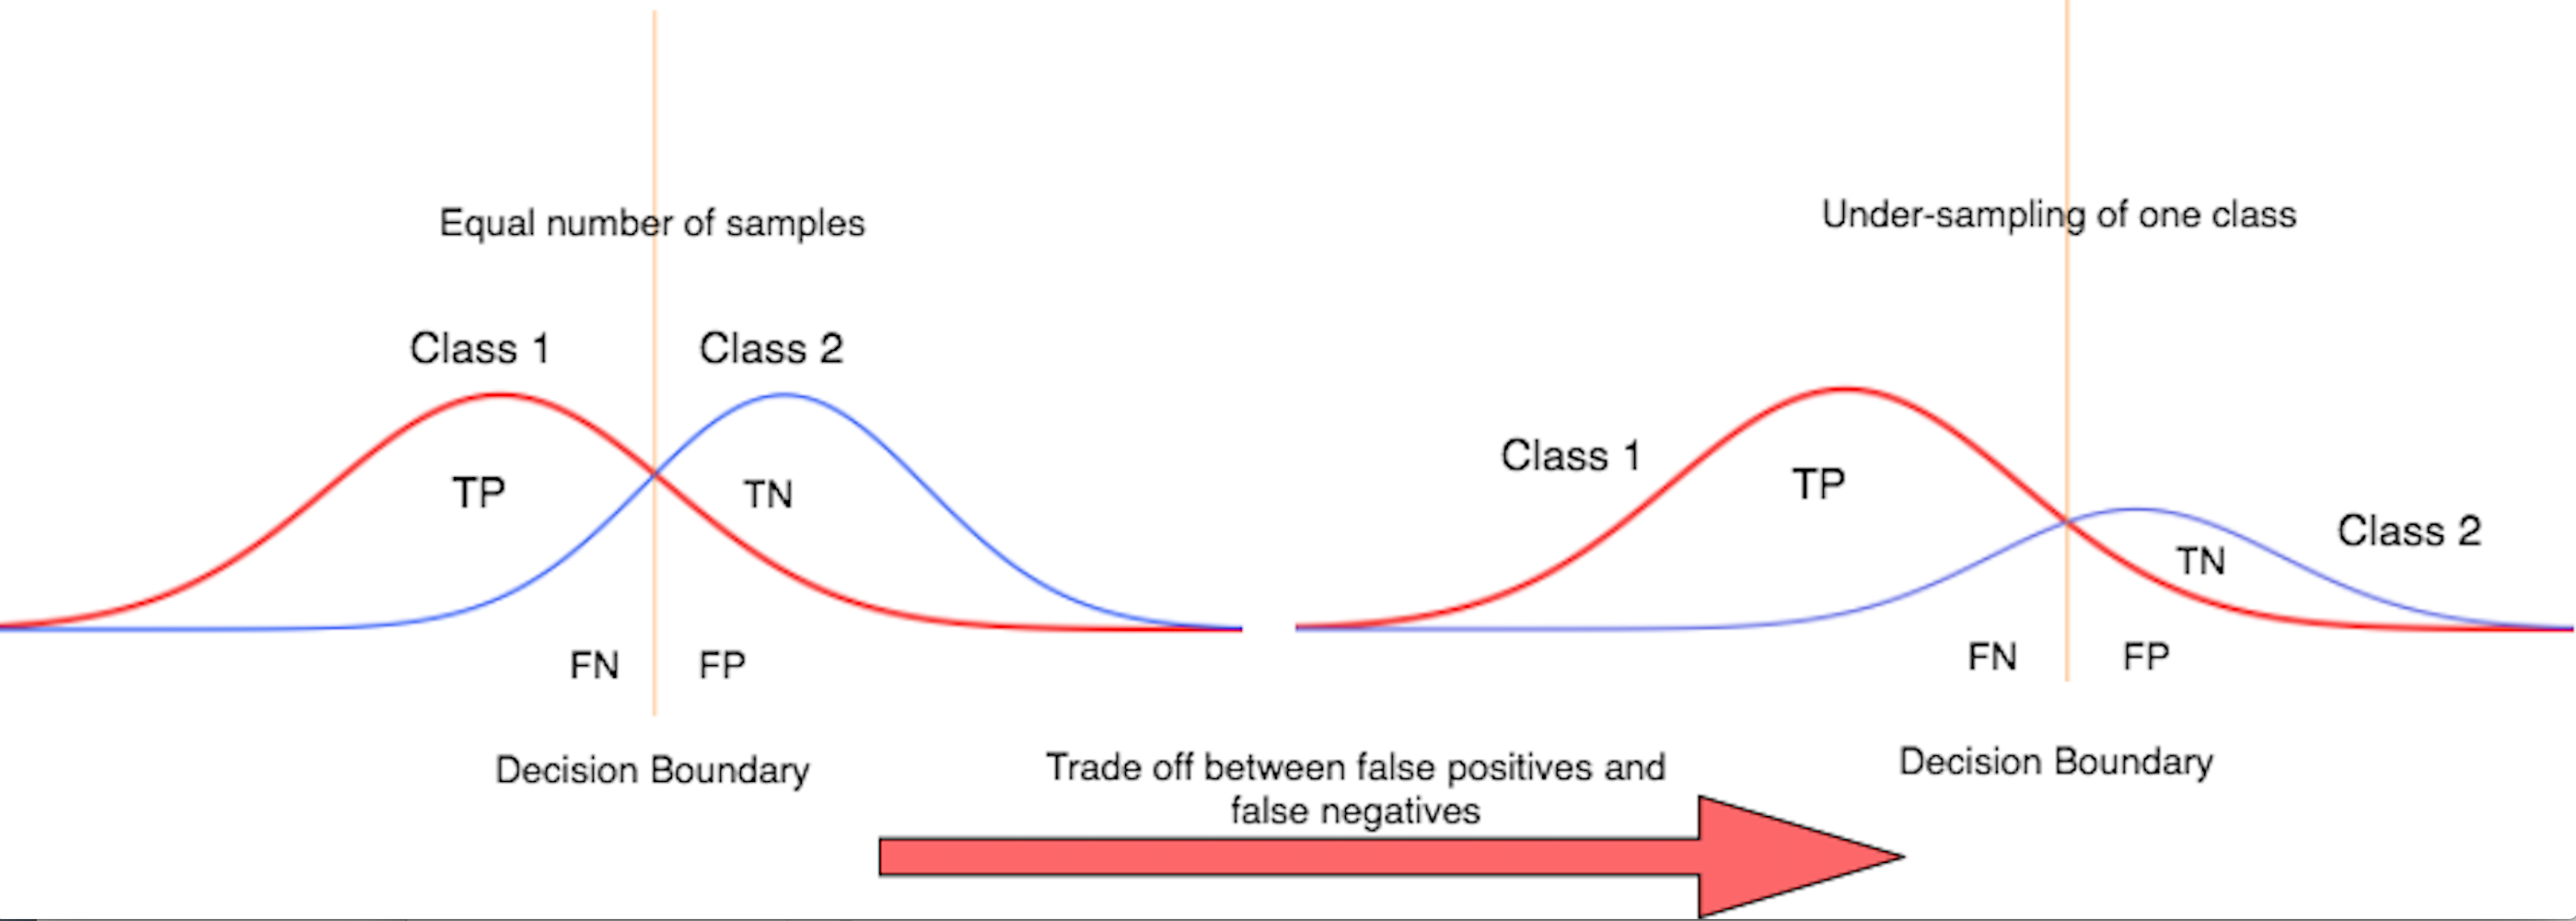
\includegraphics[height=3.5cm]{class_dist.png}
	\caption{Dataset imbalance causes models to perform adjustments of decision boundaries leading to an increase on accuracy of the majority class and decrease on the minority class.}
	\label{fig:class_dist}
\end{figure}

\subsubsection{Overlapping distributions} The results for the balanced model on figure~\ref{fig:conf_matrix_full} shows that for the pairs cat/dog and automobile/truck there is already a natural misclassification between one another. For instance 13\% of dog samples were misclassified as cat in the original balanced model. Our experiment demonstrates that the adversarial attacks intensify this phenomena in only one of the classes of the pair. While for both under-sampled cat and truck the number of samples misclassified with the similar class has increased, the same did not happen with dog and automobile. Figure~\ref{fig:overlap} shows that cats are increasingly misclassified as dogs when under-sampling on the cat class is used. While on the cat under-sampling case the percentage of samples misclassified as dogs increased from 31\% to 39\%, the same number decreased from 38\% to 32\% on the dog under-sampling test.
\begin{figure}
	\centering
	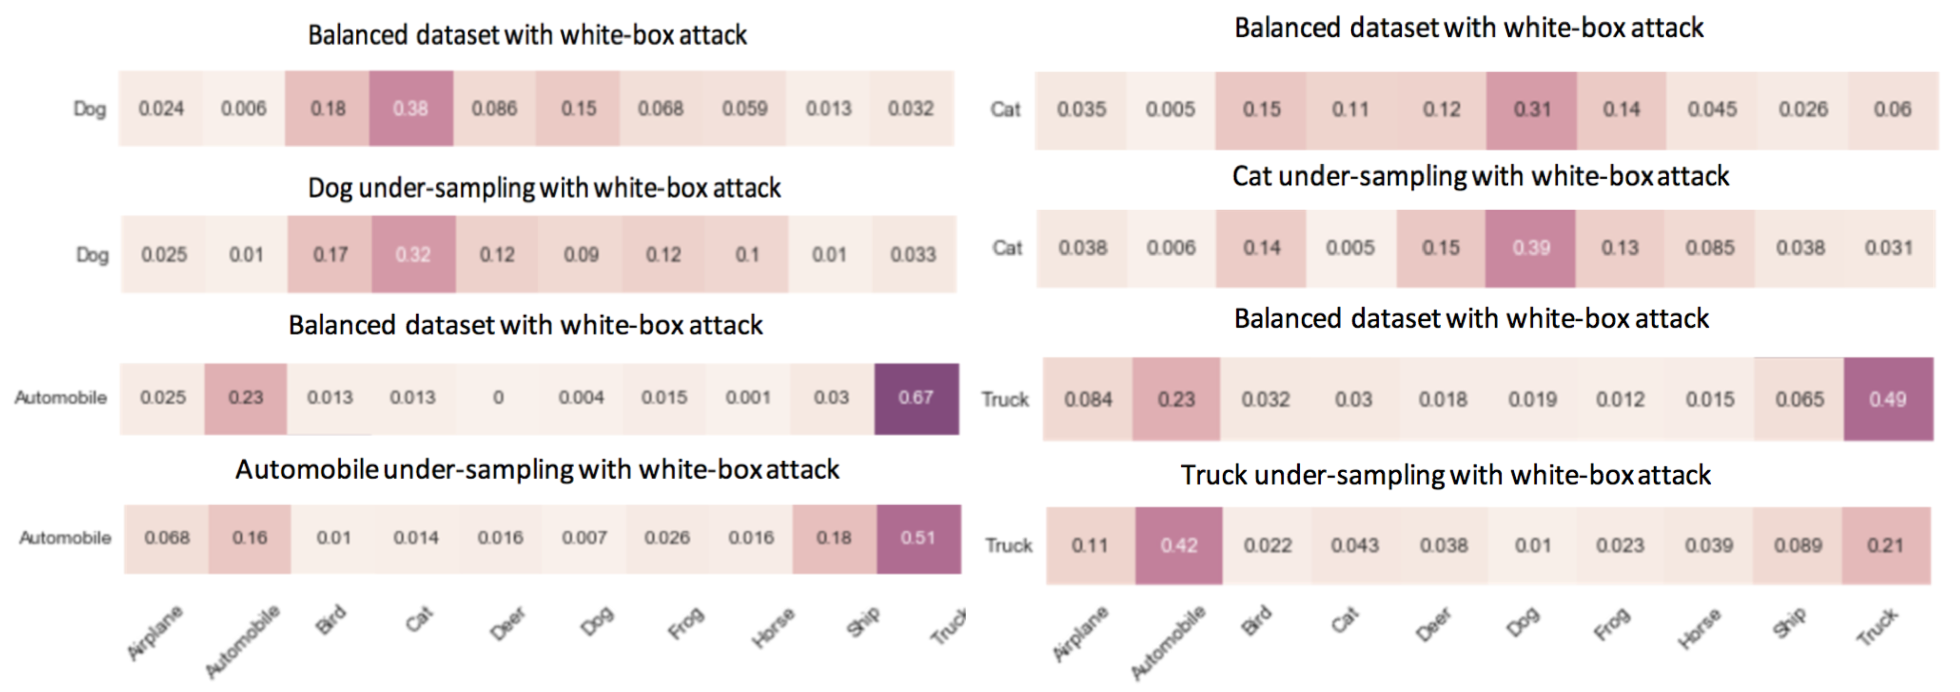
\includegraphics[height=4.5cm]{overlapping_all.png}
	\caption{Under-sample on cat and truck increases misclassification to similar classes, while dog and automobile does not.}
	\label{fig:overlap}
\end{figure}
\section{Conclusion and Future Work}

We have shown that adversarial attacks are even more severe on datasets with under-sampled class labels and that the decision boundary trade-off on the over-sampled classes increases their robustness to such attacks. Labels with similar features have only shown higher vulnerability to the fast gradient sign methods in one of the classes of the pair. This specific result shows that similar classes might have degrees of similarities on which could be more or less exploited by the gradient method.  

As several commercial applications rely on almost the same group of models, understanding of such properties is of extreme importance. Future work in this field could look further in datasets with a higher number of classes and more complex relationships between labels so as to not only confirm our insights but also discover new interesting properties of class imbalanced CNNs and adversarial attacks. Current applications looking to increase their robustness to the adversarial methods presented in this work can use over-sampling techniques on critical labels so as to shield that label from gradient sign adversarial attacks.

\bibliographystyle{splncs03}
\bibliography{refs}
\end{document}
